
\documentclass[tikz,border=6pt]{standalone}
\usepackage{tikz}
\usepackage{xcolor}
\usepackage{helvet}
\usepackage{microtype}
\renewcommand{\familydefault}{\sfdefault}
\usetikzlibrary{calc,positioning,arrows.meta}

% Palette tuned to match Futurevision.pdf
\definecolor{titleblue}{RGB}{120,145,195}
\definecolor{lineblue}{RGB}{120,145,205}
\definecolor{slate}{RGB}{90,100,115}
\definecolor{ink}{RGB}{35,35,45}
\definecolor{magentaA}{RGB}{155,60,145}

\definecolor{warmA}{RGB}{252,208,146}
\definecolor{warmB}{RGB}{250,197,132}
\definecolor{warmC}{RGB}{248,186,120}
\definecolor{warmCenter}{RGB}{244,168,92}
\definecolor{coolA}{RGB}{175,205,245}
\definecolor{coolB}{RGB}{165,195,240}
\definecolor{coolC}{RGB}{185,210,245}

\begin{document}
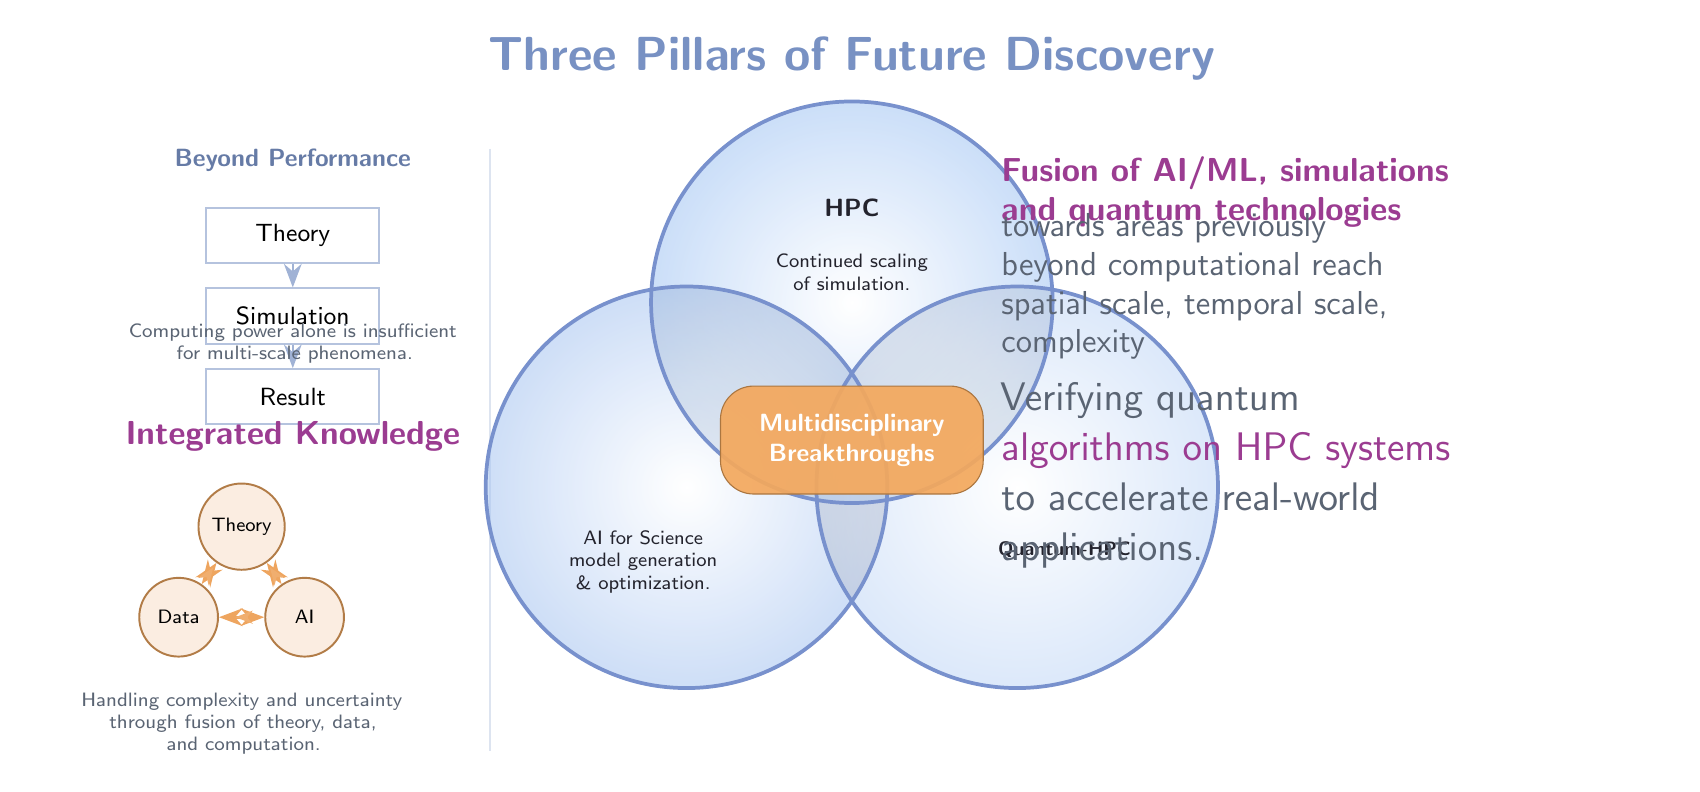
\begin{tikzpicture}[
  font=\sffamily,
  >={Stealth[length=3mm]},
  small/.style={font=\scriptsize, text=slate},
  captionstyle/.style={font=\scriptsize, text=ink},
  head/.style={font=\small\bfseries, text=ink},
  box/.style={draw=titleblue!55, line width=0.7pt, fill=white,
              minimum width=22mm, minimum height=7mm},
]

% ---- Layout bounds (roughly matching the provided slide) ----
% (No logos/footers; no parentheses text per your earlier edits)

% Title
\node[font=\LARGE\bfseries, text=titleblue] at (0,4.25)
{Three Pillars of Future Discovery};

% =========================
% LEFT COLUMN
% =========================
\node[head, align=center, text=titleblue!85!black] at (-7.10,2.95)
{Beyond Performance};

% Old model flow chart
\node[box] (th)  at (-7.10,2.00) {\small Theory};
\node[box, below=3mm of th] (si) {\small Simulation};
\node[box, below=3mm of si] (re) {\small Result};

\draw[->, line width=0.9pt, titleblue!70] (th) -- (si);
\draw[->, line width=0.9pt, titleblue!70] (si) -- (re);

\node[small, align=center, text width=50mm] at (-7.10,0.62)
{Computing power alone is insufficient\\ for multi-scale phenomena.};

\node[font=\large\bfseries, text=magentaA, align=center] at (-7.10,-0.55)
{Integrated Knowledge};

% Bottom-left mini-network (Theory/Data/AI) with orange arrows
\definecolor{arrowOrange}{RGB}{238,165,95}
\definecolor{nodeOrange}{RGB}{244,205,170}

\node[draw=arrowOrange!75!black, fill=nodeOrange!35, line width=0.7pt,
      circle, minimum size=10mm] (T)  at (-7.75,-1.70) {\scriptsize Theory};
\node[draw=arrowOrange!75!black, fill=nodeOrange!35, line width=0.7pt,
      circle, minimum size=10mm] (D)  at (-8.55,-2.85) {\scriptsize Data};
\node[draw=arrowOrange!75!black, fill=nodeOrange!35, line width=0.7pt,
      circle, minimum size=10mm] (A)  at (-6.95,-2.85) {\scriptsize AI};

\draw[<->, line width=1.0pt, arrowOrange] (T) -- (D);
\draw[<->, line width=1.0pt, arrowOrange] (T) -- (A);
\draw[<->, line width=1.0pt, arrowOrange] (D) -- (A);

% small "fusion" arrows (stylized)
\foreach \p/\q in {T/D,T/A,D/A}{
  \draw[-{Stealth[length=2.2mm]}, line width=0.8pt, arrowOrange!90]
    ($(\p)!0.55!(\q)$) -- ($(\p)!0.45!(\q)$);
}

\node[small, align=center, text width=52mm] at (-7.75,-4.20)
{Handling complexity and uncertainty\\ through fusion of theory, data,\\ and computation.};

% subtle divider line (as in slide)
\draw[titleblue!25, line width=0.7pt] (-4.60,3.10) -- (-4.60,-4.55);

% =========================
% CENTRAL VENN (with gradients)
% =========================
\coordinate (Ctop)   at (0,1.15);
\coordinate (Cleft)  at (-2.10,-1.20);
\coordinate (Cright) at ( 2.10,-1.20);
\def\R{2.55}

% Pairwise overlaps + triple overlap (soft fills)
\begin{scope}
  \clip (Ctop) circle (\R);
  \fill[warmA, opacity=0.55] (Cleft) circle (\R);
\end{scope}
\begin{scope}
  \clip (Ctop) circle (\R);
  \fill[warmB, opacity=0.55] (Cright) circle (\R);
\end{scope}
\begin{scope}
  \clip (Cleft) circle (\R);
  \fill[warmC, opacity=0.55] (Cright) circle (\R);
\end{scope}
\begin{scope}
  \clip (Ctop) circle (\R);
  \clip (Cleft) circle (\R);
  \clip (Cright) circle (\R);
  \fill[warmCenter, opacity=0.78] (-6,-6) rectangle (6,6);
\end{scope}

% Radial gradient shading inside each circle (gives the "glow" look)
% Top circle
\begin{scope}
  \clip (Ctop) circle (\R);
  \shade[inner color=white, outer color=coolA, opacity=0.65]
    (Ctop) circle (\R);
\end{scope}
% Left circle
\begin{scope}
  \clip (Cleft) circle (\R);
  \shade[inner color=white, outer color=coolB, opacity=0.55]
    (Cleft) circle (\R);
\end{scope}
% Right circle
\begin{scope}
  \clip (Cright) circle (\R);
  \shade[inner color=white, outer color=coolC, opacity=0.50]
    (Cright) circle (\R);
\end{scope}

% Outlines (thick, bluish)
\draw[line width=1.35pt, lineblue] (Ctop)   circle (\R);
\draw[line width=1.35pt, lineblue] (Cleft)  circle (\R);
\draw[line width=1.35pt, lineblue] (Cright) circle (\R);

% Labels (no parentheses)
\node[align=center, font=\small\bfseries, text=ink] at ($(Ctop)+(0,1.20)$) {HPC};
\node[captionstyle, align=center] at ($(Ctop)+(0,0.38)$) {Continued scaling\\ of simulation.};

\node[captionstyle, align=center] at ($(Cleft)+(-0.55,-0.95)$)
{AI for Science\\ model generation\\ \& optimization.};

\node[captionstyle, align=center] at ($(Cright)+(0.60,-0.80)$)
{\textbf{Quantum-HPC}};

% Center badge
\node[
  draw=warmCenter!70!black,
  fill=warmCenter,
  fill opacity=0.92,
  text opacity=1,
  rounded corners=12pt,
  inner xsep=14pt,
  inner ysep=10pt,
  align=center,
  font=\small\bfseries,
  text=white
] at (0,-0.60) {Multidisciplinary\\ Breakthroughs};

% =========================
% RIGHT COLUMN TEXT
% =========================
\node[align=left, text width=84mm, font=\large\bfseries, text=magentaA] at (6.10,2.55)
{Fusion of AI/ML, simulations\\ and quantum technologies};

\node[align=left, text width=84mm, font=\large, text=slate] at (6.10,1.35)
{towards areas previously\\ beyond computational reach\\
spatial scale, temporal scale,\\ complexity};

\node[align=left, text width=84mm, font=\Large, text=slate] at (6.10,-1.05)
{Verifying quantum\\
\textcolor{magentaA}{algorithms on HPC systems}\\
to accelerate real-world\\ applications.};

\end{tikzpicture}
\end{document}
